\section{Tabular Reinforcement Learning}

Trajectory: $\tau \defeq (\tau_0, \tau_1, \dots)$, with $\tau_i \defeq (x, a, r, x')$ \\
\textbf{on-policy}: Agent learns while following policy \\
\textbf{off-policy}: Agent can follow any policy \\
\textbf{Model-based} $\rightarrow$ Learn the underlying MDP \\
\textbf{Model-free} $\rightarrow$ Learn the value function directly.
\begin{framed}
    If model-based, MLE is ${\hat{p}(x' \mid x, a) = \frac{N(x' \mid x, a)}{N(a \mid x)}}$ and ${\hat{r}(x, a) = \frac{1}{N(a \mid x)} \sum_{t = 0}^\infty r_t}$
\end{framed}
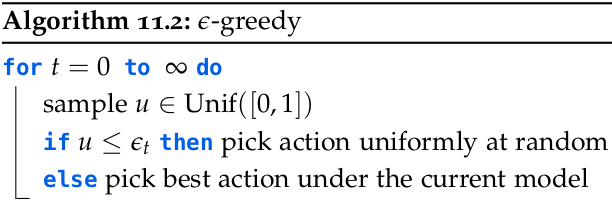
\includegraphics[width=0.9\linewidth]{images/epsilon_greedy.png}
$\epsilon$-greedy Monte Carlo converges, e.g., for $\epsilon_t = \frac{1}{t}$
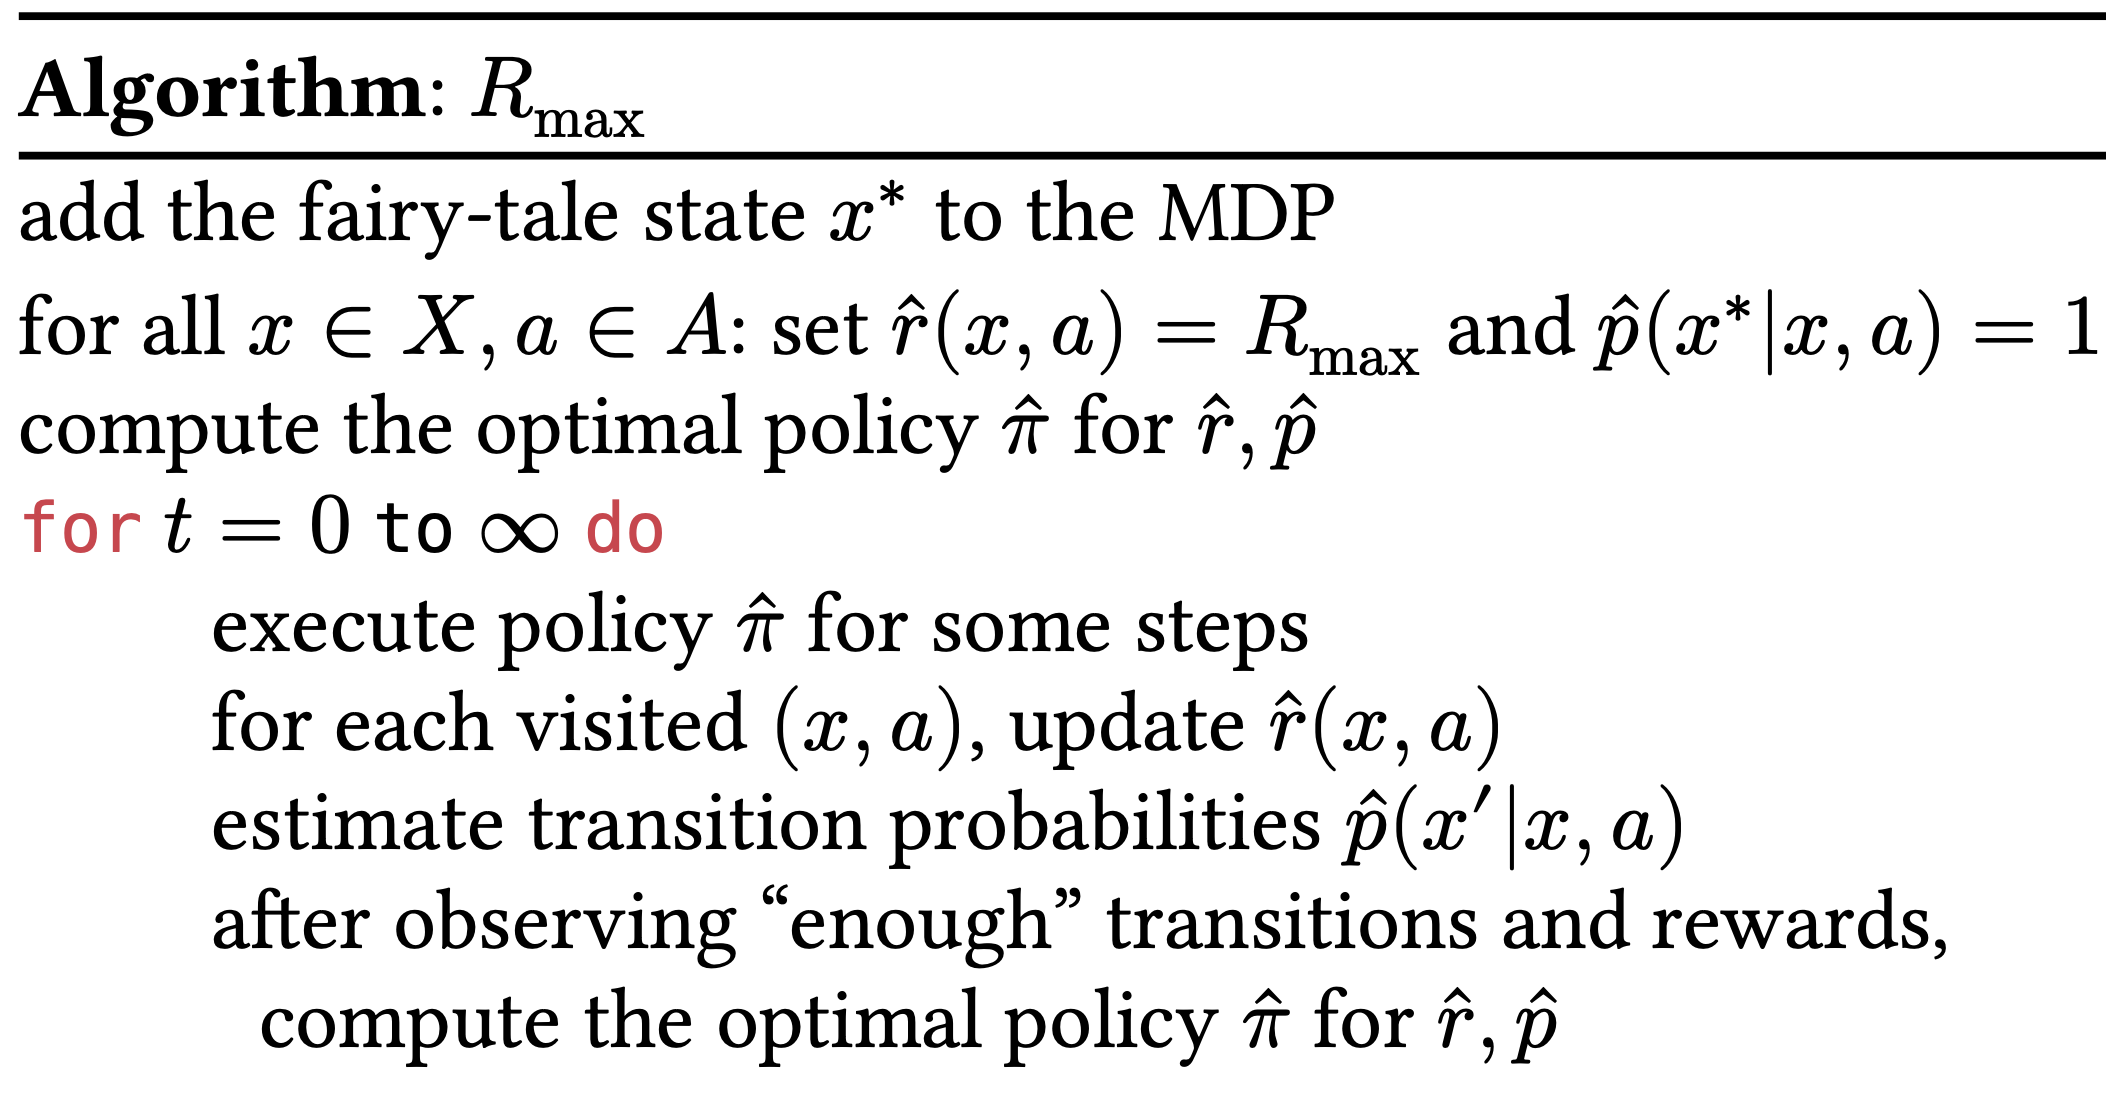
\includegraphics[width=0.95\linewidth]{images/R_max.png}
With probability $\geq 1-\delta$, $R_\mathrm{max}$ reaches an $\epsilon$-optimal policy in a no. of steps polynomial in $\card{\sX}$, $\card{\sA}$, $T$, $\nicefrac{1}{\epsilon}$, $\nicefrac{1}{\delta}$, and $R_\mathrm{max}$.
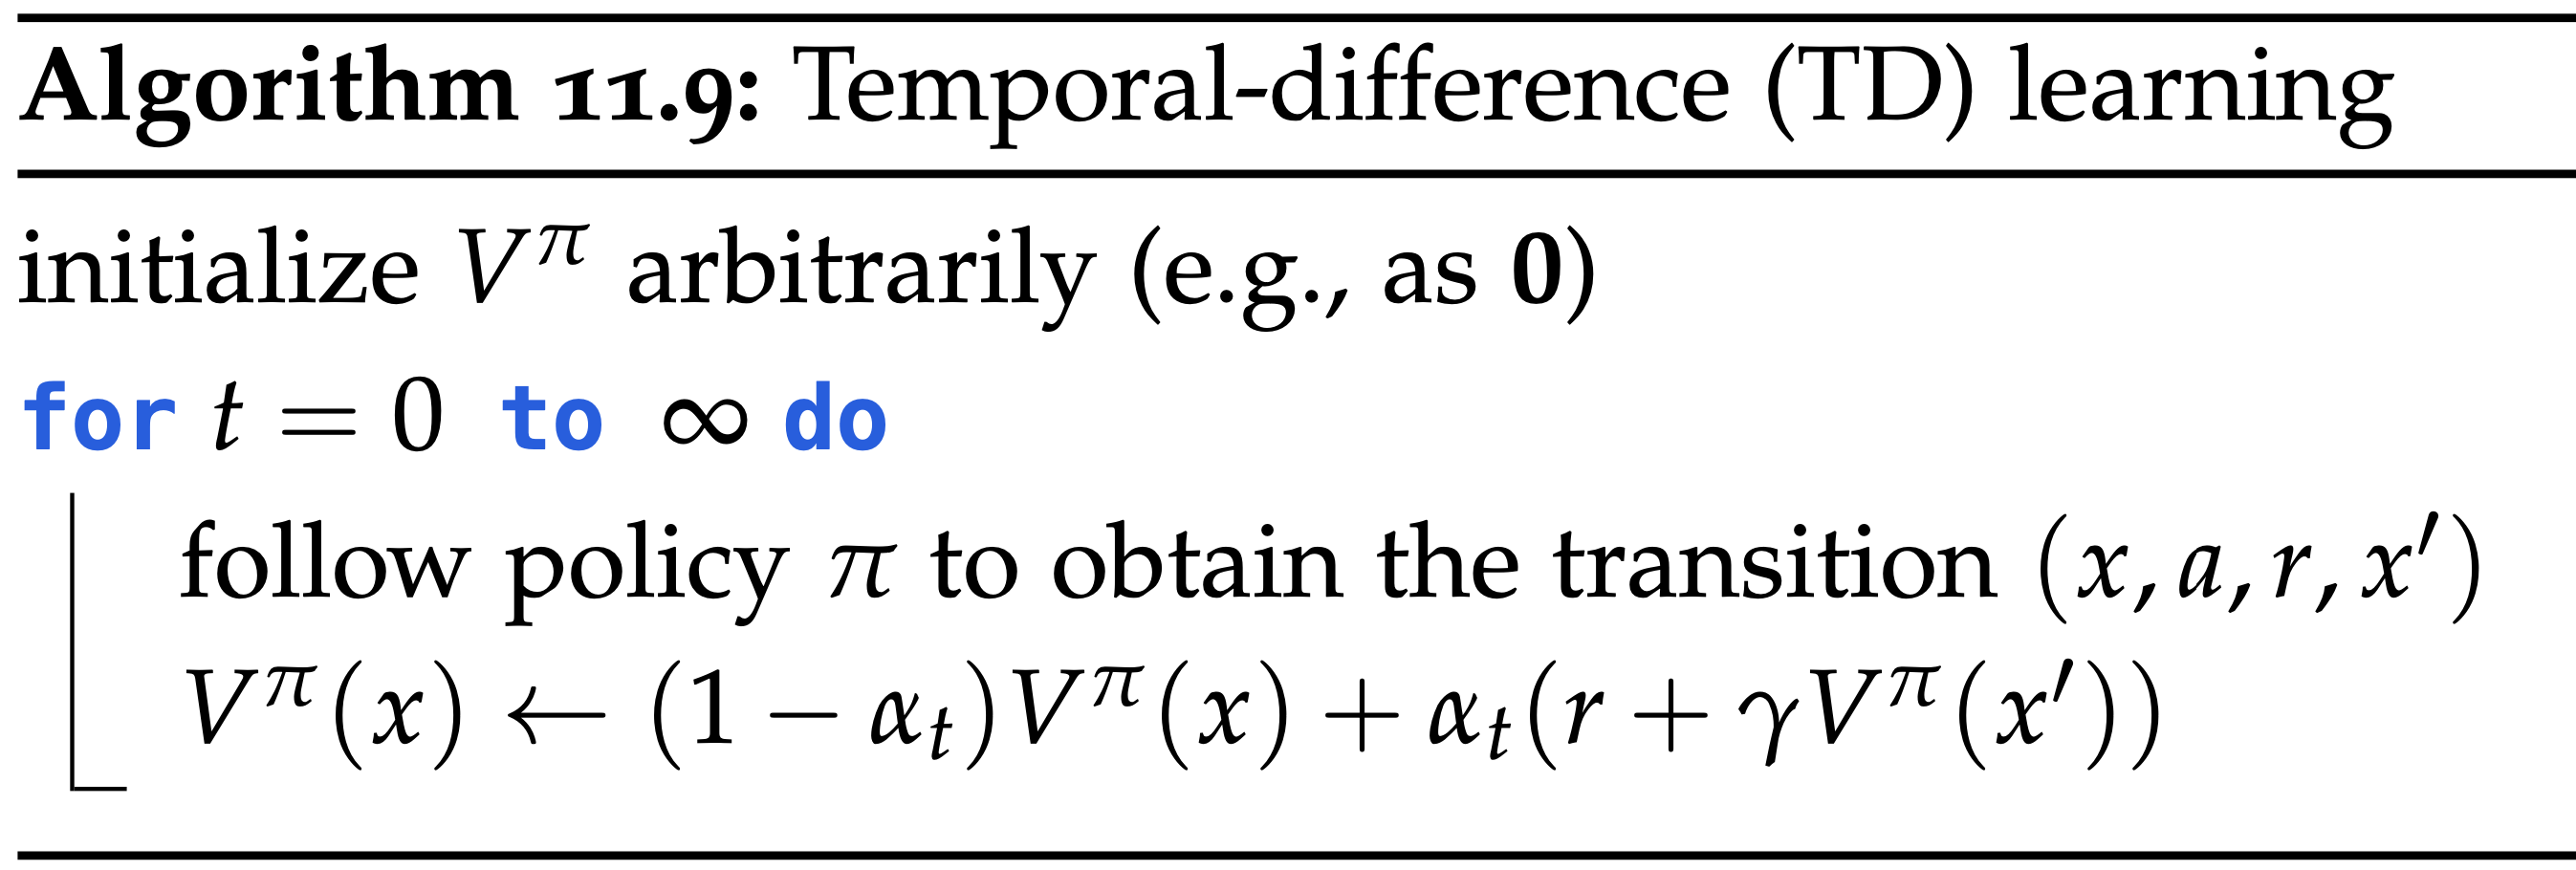
\includegraphics[width=0.95\linewidth]{images/TD_learning.png}
TD is model-free and on-policy.
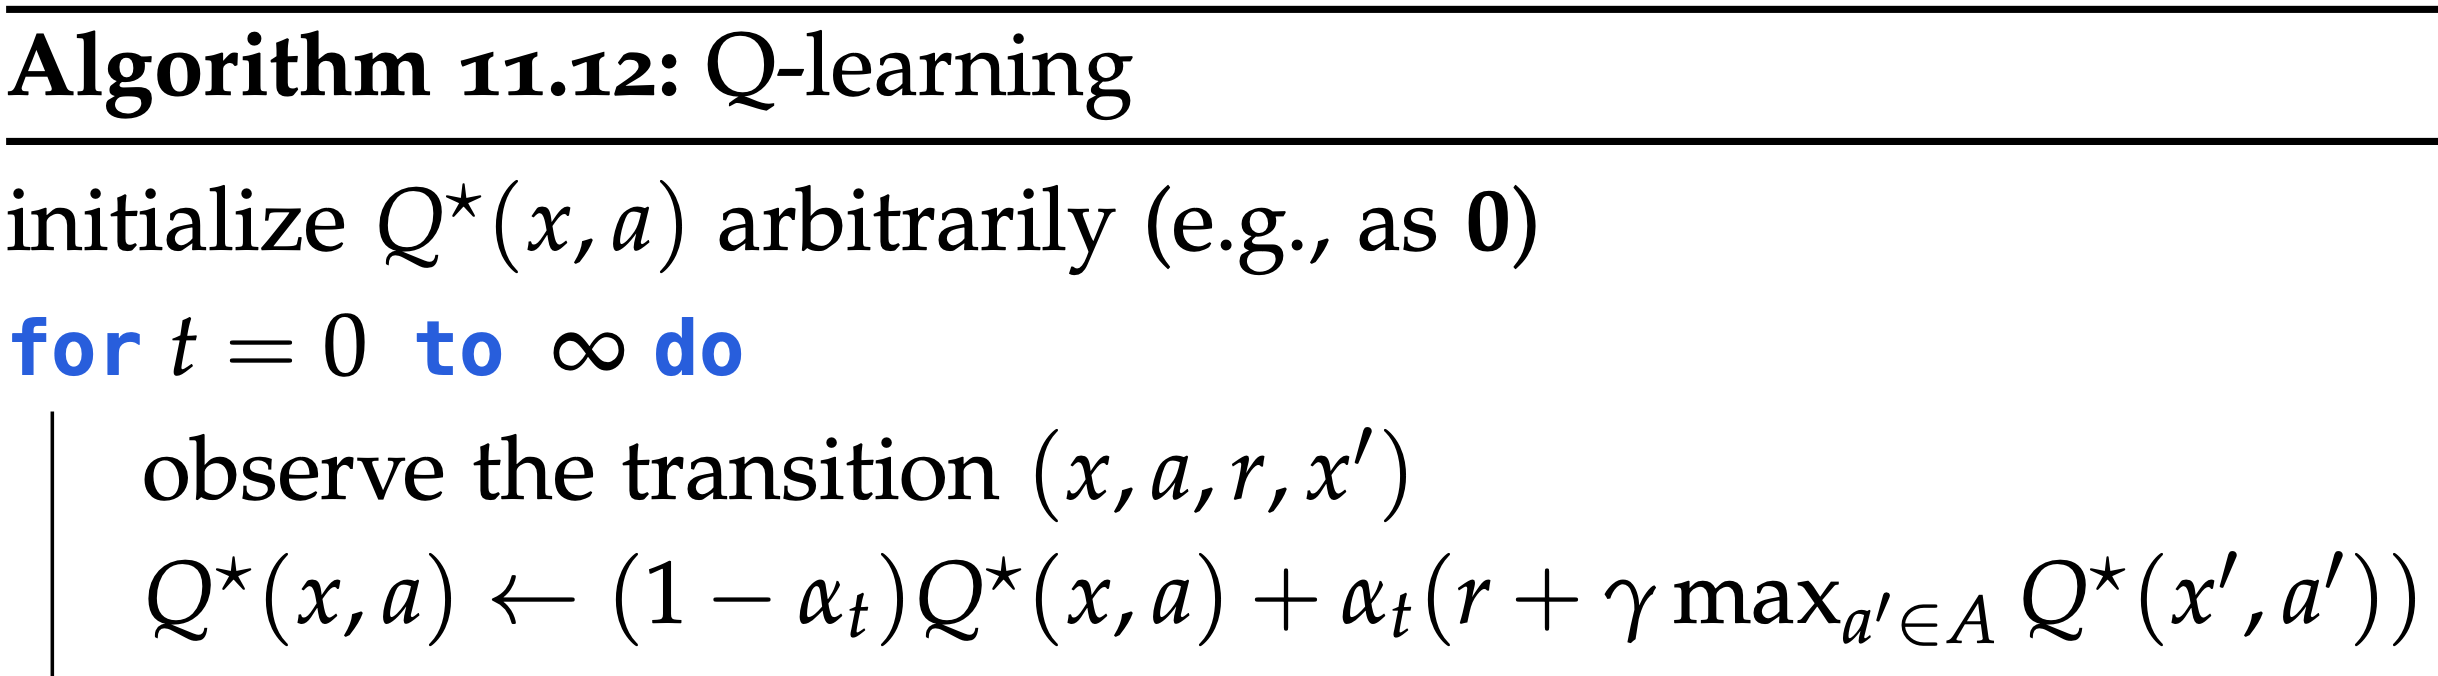
\includegraphics[width=0.95\linewidth, trim={0 0 1cm 0}]{images/Q_learning.png}
Q is model-free \& off-policy, $\BigO{nm}$ memory. \\
Alt. update: $\Q*{x}{a} \gets \Q*{x}{a} + \alpha_t\parentheses*{r + \gamma \max_{a' \in \sA} \Q*{x'}{a'} - \Q*{x}{a}}$. \\
Variant: \textbf{Optimistic Q-Learning}, $V_{\max} = \frac{R_{\max}}{1-\gamma}$. Init. $Q(x, a) = V_{\max} \prod_{t=0}^{T_{\text{init}}} (1-\alpha_t)^{-1}$. Pick $a_t = \argmax_a Q(x_t, a)$.
\begin{framed}
    \textbf{RM cond.}: $\alpha_t \geq 0, \sum_{t=0}^{\infty}{\alpha_t} = \infty, \sum_{t=0}^{\infty}{\alpha_t^2} < \infty$. \\
\end{framed}
If $\alpha_t$ satisfy RM conditions and every state-action pair is visited infinitely often (=sample inefficient), then we have convergence for \{TD, $Q$, $Q_{\text{Opt}}$\} learning.
